\documentclass[tikz,14pt]{article}

% Math
\usepackage[fleqn]{amsmath}
\usepackage{amssymb}
\usepackage{dsfont}
\usepackage{float}


% Allows to use caption*
\usepackage{caption}
% Scalabale subfigures
\usepackage{subcaption} 
% Code syntax highlighting
\usepackage{minted}
% Hyperlinks
\usepackage{hyperref}


\newcommand{\bmat}[1]{
   \ensuremath{
   \begin{bmatrix}
       #1
   \end{bmatrix}
}}



\usepackage[utf8]{inputenc}
\usepackage[margin=1in]{geometry}
\usepackage[titletoc,title]{appendix}
\usepackage[dvipsnames]{xcolor}
\usepackage{latexsym}
\usepackage{multicol}
\usepackage{graphicx}
\usepackage{fancyhdr}
\usepackage[linguistics]{forest}
\usepackage{colortbl}
\usepackage{pdfpages}
\usepackage{wrapfig}
\usepackage{dirtree}
\usepackage{xifthen}% provides \isempty test
\usepackage{glossaries}
\usepackage{pgfplots}

\definecolor{darkblue}{rgb}{0.0, 0.0, 1}
\usepackage[pdftex,hyperfigures,hyperindex,bookmarksnumbered,colorlinks, bookmarks, breaklinks, linktocpage,citecolor=darkblue,urlcolor=darkblue,linkcolor=darkblue,pagebackref=true]{hyperref}

% to fixme
\definecolor{FIXMECOLOR}{rgb}{1,0,0.3}
\newcommand{\FIXME}[1]{{\color{FIXMECOLOR}{\textbf{FIXME: #1}}}} 

% code blocks
\definecolor{LightGray}{gray}{0.95}
\usepackage{minted}
\setminted[]{
    frame=lines,
    framesep=2mm,
    baselinestretch=1.2,
    bgcolor=LightGray,
    fontsize=\small,
    linenos,
    mathescape=true,
    escapeinside=||,
}


\definecolor{color1}{HTML}{0B0C10}
\definecolor{color2}{HTML}{1F2833}
\definecolor{color3}{HTML}{C5C6C7}
\definecolor{color4}{HTML}{66FCF1}
\definecolor{color5}{HTML}{45A29E}

\pagestyle{fancy}
\fancyhf{}
%%%%%%%%%%%%%%%%%%%%%%%%%%%%
%% VARIABLES
\newcommand\sitename{Banana\texttrademark}
\newcommand\assignmenttitle{Project Report}
\newcommand\namesurname{Albert Cerfeda\\Alessandro Gobbetti}
\newcommand\assignment{}

\newcommand\subject{Information Retrieval}
\newcommand\documentdate{16.12.2022}

% Title content
%%%%%%%%%%%%%%%%%%%%%%%%%%%%
\rhead{\assignment}
\lhead{\namesurname}
%%%%%%%%%%%%%%%%%%%%%%%%%%%%
\rfoot{Page \thepage}
\setlength{\parindent}{0pt}

\newcommand\xdownarrow[1][2ex]{%
   \mathrel{\rotatebox{90}{$\xleftarrow{\rule{#1}{0pt}}$}}
}

\begin{document}

\begin{titlepage}
   \begin{center}
       \vspace*{1cm}

       \textbf{\Large{\assignmenttitle}}

       \vspace{0.5cm}
        \textbf{\subject}\\[5mm]
       \assignment
        
            
       \vspace{1.1cm}

        \namesurname\\
        \vspace{1cm}

        This project was realized in the span of about 2 weeks (14 days).\\
Developed as part of the group project for \textit{Information Retrieval SA 2021-2022}, part of BSc INF at Università della Svizzera Italiana (USI) in Lugano.
       \tableofcontents
       

       \vspace*{\fill}
     
       \includegraphics[width=0.4\textwidth]{fig/logo.pdf}
       
        \documentdate \\
        Università della Svizzera italiana\\
        Faculty of Informatics\\
        Switzerland\\

   \end{center}
\end{titlepage}

%%%%%%%%%%%%%%%%%%%%%%%%%%%%%%%%%%%%%%%%%%%%%%%%%%%%
%%%%%%  CONTENT START   %%%%%%%%%%%%%%%%%%%%%%%%%%%%
% color	white, black, red, green, blue, cyan, magenta, yellow
% thickness	ultra thin, very thin, thin, thick, very thick, ultra thick
% dots (/loosely/densely) + dotted, dashed, dashdotted


\section{Introduction} \label{sec:intro}
\textbf{\sitename\footnote{Banana is not an actual trademark. We thought it was funny xd}} aims to be a search engine to discover and fund your favourite content creators.\\
We put efforts into making our system sustainable and self-improving, without requiring us to start processes or intervene manually. We faced quite a lot of challenges, mostly regarding Solr [See Sec.\ref{sec:solr}] and its very steep learning curve.\\
Nonetheless, we are satisfied enough with the current state of the project. There are still many improvements to be done, but considering the time on our hands this is good enough.\\


\section{Tech stack} \label{sec:stack}
\begin{figure}[h!]
    \includegraphics*[width=\linewidth]{fig/StackDiagram.png}
\end{figure}
In our system there are dfferent components that operate independently from one another. It's important to gain understanding of the moving pieces that make our system work.

\subsection{Scrapy} \label{sec:scrapy}
Scrapy is an open source Python framework for crawling and scraping websites \footnote{Scrapy: See \href{https://scrapy.org}{website}}. Our backend invokes the Scrapy process for crawling/scraping a set of artists, categories or search queries. The scraped data output is then directed into a \verb|.json| file, ready to be read and indexed by Solr.

\subsection{Solr} \label{sec:solr}
Solr is a popular enterprise search platform built on top of \textit{Apache Lucene}\footnote{Solr: See \href{https://solr.apache.org/guide/solr/9_0/index.html}{website}}. It includes features like distributed indexing, replication and load-balanced querying, and automatic recovery.\\
It is responsible for indexing and querying the collection. It retrieves the artists most pertinent to the user's search query and filters.

\subsection{NodeJS + MongoDB} \label{sec:node-mongo}
For our backend we chose NodeJS \verb|v. 19.2.0|. It handles user queries, relevance feedback and coordinates and interacts with all the other components of our stack.\\
It also handles the scraping and indexing process, as it periodically provides the Solr and Scrapy processes with the authors/tags/queries to scrape and index. The MongoDB database serves for the purpose of storing and remembering the index timestamp for each author/tag/query.\\
The user has the option to label as "unsatisfying" the search results for a query: the backend will then instruct Scrapy to scrape the search results of each site for the provided user query.\\
It performs additional computation on the user's query such as pagination, query reranking, sorting, "more like this" similarity feature and input sanification.\\ It also adopts some security measures like using a rate limiter to protect from DDOS attacks. See Section \ref{sec:backend} for a more detailed explanation of how the backend works.

\subsection{Vue.js 3} \label{sec:vuejs}
The frontend plays the crucial part of presenting the retrieved documents. 
It is responsible for the user interface, the user experience and the interaction with the backend. 
It is built with Vue.js 3, using Vuetify 3 as a UI library. Vue.js allows us to create a reactive and dynamic user interface, while Vuetify provides us with a set of pre-built components and styles.\\
During the development of the frontend, we discover that the Vuetify library is not yet fully finished and stable. This caused us some problems, but we managed to overcome them.\\


\section{Retrieving and indexing documents} \label{sec:retrieving}
Retrieving and indexing documents is the core of any search engine. In this section we will describe these two processes in detail.




\subsection{Crawling process} \label{sec:crawling}
Retrieving documents from the web is a complex process. 
The crawling process is used to retrieve documents from the web.
This is done by a crawler (also called spider), that automatically visit web pages and read their content.
When a crawler visits a web page, it extracts the links to other pages and adds them to the list of pages to visit.
This process is repeated until the crawler has visited all the pages it can find.
In the case of our project, we used the \href{https://scrapy.org/}{Scrapy framework} to crawl the web pages.

In order to properly crawl a website we need to understand how it is structured.
For this reason, this was a fundamental part in the project to decide which sites to crawl.
Some websites are not meant to be crawled easily.

An ideal website to crawl would have a list of links to all the pages to crawl (all the creators using the site).
\href{https://www.subscribestar.com/stars?_page=true&page=1}{SubscibeStar} is a perfect example of this:
the whole website is static and the creators are listed. 
The only thing to do is visit every site in the list on every page and extract the information.
This is not the case for most websites, and we had to find a way to crawl them.


\href{https://www.ko-fi.com/}{Ko-fi}, for example, does not list all the creators, so we had to find another way to crawl it.
Since creators have tags associated with them, we decided to use them and search by category.

\href{https://www.patreon.com/}{Patreon} does not even have categories, 
so we decided to query the site using random super-generic keywords (like "music" or "art").
This way we are not sure to find all the creators, but at least we can crawl a lot of them.

The crawling process is not always straightforward, and we had to make some compromises.
When we crawl a website we are sending thousands of requests to a webserver, and we need to be careful not to overload it or get banned.
Some websites have a limit on the number of requests per second.
Between the three websites we crawled, href{https://www.ko-fi.com/}{Ko-fi} has the most restrictive policy.

We used some good practices to safely crawl the websites. To avoid sending too many requests at the same time, we used a delay between requests.
For the case of href{https://www.ko-fi.com/}{Ko-fi}, we set the \mintinline{python}{DOWNLOAD_DELAY} to 3 seconds,
which means that the crawler will wait a random interval between $0.5 \cdot 3$ and $1.5 \cdot 3$ seconds 
before sending the next request since the \mintinline{python}{RANDOMIZE_DOWNLOAD_DELAY} setting is enabled (by default).

Another good practice is to use a \textit{user agent} to identify the crawler.
This is a string that is sent with every request, and it is used by the webserver to identify the client.
The \textit{user agent} contains information about the client, like the operating system, the browser, and the version.
To be more clear, an example of user agent is: 
\begin{minted}[fontsize=\footnotesize]{bash}
Mozilla/5.0 (X11; Linux x86_64) AppleWebKit/537.36 (KHTML, like Gecko) Chrome/107.0.0.0 Safari/537.36
\end{minted}
At every request, thanks to the \mintinline{python}{scrapy.downloadermiddlewares.useragent.UserAgentMiddleware} middleware
our crawler uses a random user agent.

Another problem we faced is that some websites are javascript-heavy, so we had to wait some time for the page to load.
To solve this problem, we used the \verb|scrapy-playwright| library, which is a middleware that uses the \href{https://playwright.dev/}{Playwright} library to interact with the browser.
It simulates a real user using a real browser, so it can wait for the page to load and interact with it. 
We used it to wait until a css selector was present on the page, but it can do much more, like clicking on buttons or filling forms.

The spiders we coded have a common structure, they can take as parameter a list of tags to search, 
a list of urls of creators pages, or a list of queries to perform on the website.
The default parameters are used when we want to crawl the whole website.
The spiders have a method \mintinline{python}{parse} that is called on the pages listing artists.
This method extracts the urls of the artists pages and calls the \mintinline{python}{parse_artist} method on them.
It also extracts the urls of the next pages and calls itself on them.
The \mintinline{python}{parse_artist} method is the one that extracts the information from the artist page.
All the information are stored in the same format tanks to the \mintinline{python}{artist_dict.make} method.
The info we save for each artist are:
\begin{itemize}
    \item \mintinline{python}{site}: the website we crawled (ko-fi, patreon, subscribestar)
    \item \mintinline{python}{page_link}: the url of the artist page
    \item \mintinline{python}{artist_name}: the name of the artist
    \item \mintinline{python}{artist_image}: the url of the artist image
    \item \mintinline{python}{artist_banner}: the url of the artist banner
    \item \mintinline{python}{bio}: a short description of the artist
    \item \mintinline{python}{bio_long}: a more detailed description of the artist
    \item \mintinline{python}{amount_post}: the number of posts the artist has
    \item \mintinline{python}{amount_subs}: the number of subs the artist has
    \item \mintinline{python}{price_tiers_title}: a list of all the price tiers titles
    \item \mintinline{python}{price_tiers_monthly}: a list of strings of all the price tiers amounts per month
    \item \mintinline{python}{price_tiers_monthly_chf}: a list of all the price tiers amounts converted to CHF
    \item \mintinline{python}{price_tiers_description}: a list of all the price tiers descriptions
    \item \mintinline{python}{tags}: a list of tags associated with the artist
    \item \mintinline{python}{socialmedias}: a list of social media links
    \item \mintinline{python}{indexDate}: the date of the crawling
\end{itemize}

All the crawled data can be outputted by scrapy in a json file, that we use in the next section to index the data.

To run the spiders, navigate to the \mintinline{bash}{crawler/crawler} folder and run the following command:
\begin{minted}{bash}
scrapy crawl <spider-name> [OPTIONAL PARAMETERS] -o outputfile.json
\end{minted}
where \mintinline{bash}{<spider-name>} is the name of the spider you want to run,
and \mintinline{bash}{outputfile.json} is the name of the file where the data will be saved.

The optional parameters can be passed as \mintinline{bash}{-a tags=[...] -a artists=[...] -a searches=[...]}.



\subsection{Indexing process} \label{sec:indexing}
Once the data are crawled, we need to index it to then be able to find the documents that match a query.
We use the Apache Solr search engine to do so, which is an open-source search engine that uses the Lucene library to build an inverted index.
 
\section{The glue that keeps everything together: the backend} \label{sec:backend}
Our backend is center of operations. It starts and administers most of the processes that happen on the server, hidden from the user.

\subsection{Automatic scraping} \label{sec:scraping}
The backend relies on a MongoDB database for storing the index dates of tags and for storing the search queries searched for on the different sites.\\
All the configuration options for the backend are stored inside the \textit{config.json} file. There you can customize almost every aspect of the application, like the page size, how much time needs to pas for considering a document as expired and therefore put it up for scraping.\\

The backend uses a \textit{rate limiter} for limiting the amount of received requests, ensuring some degree of protection from DDoS attacks.

\subsection{Handling user queries} \label{sec:queries}
There are different API endpoints available to the frontend:\\
\begin{enumerate}
\item /query/feedback
With this route the user can provide explcit feedback for the search results of a query.\\
Once a user is dissatisfied with a query's search results, the query in question is saved into MongoDB to be automatically earched for and indexed for on the different sites.
\item /query/stats
This route allows the frontend to retrieve all statistics of the collection. This way the frontend can display the filters with the appropriate values and display the categories that are most popular on the homepage.
\item /query/mlt
This route is used by the frontend for retrieving artists that are similar to a set of other artist(s). We used the "More Like This" method handler in Solr.
\item /query/*
Finally the most useful route: here the user can provide search query terms and filter values and the backend answers with the ranked documents.\\
A very interesting query preprocessing is done: All the words of the query are escaped with starts (ie '*') therefore enabling partial query matching. If a user types a query term escaped with quotes (ie "quote") the backend performs an EXACT query match for those words. This feature was clearly inspired to Google's Search engine.\\
\end{enumerate}

\section{Presenting documents to users: the frontend} \label{sec:frontend}
The search engine is not the only part of an IR system, we also need to present the documents to the user and 
provide a way for them to interact with the documents, perform queries and in general brouse the system.
The frontend does it.

The homepage shown in \autoref{fig:homepage} contains a search bar where the user can type a query and press enter to perform it.
Some of the most popular tags are also shown, and the user can click on them to quickly retrieve the documents associated with them.
The user can also click on the \textit{Advanced search} button to perform a more complex query: 
a form is shown below the search bar where the user can specify the websites they want to search in,
the categories the artists must belong to, the amount of subs they must have (through a range slider), 
and a range of prices the artists must offer (through a range slider again).
The user can specify an exact match for the words in the query by putting them in double quotes, 
otherwise  
The query is performed when the user clicks enter in the search bar.


\begin{figure}[H]
    \centering
    % add box around figure
    \fbox{\includegraphics[width=0.9\linewidth]{fig/homepage.png}}
    \caption{The homepage of the website.}
    \label{fig:homepage}
\end{figure}

The results are shown in a list of cards (see \autoref{fig:resultspage}) sorted by the score of the documents, which is computed by Solr.
Each card contains the most important information about the artist and the user can click on a card to expand it 
and see more information about the artist and the price tiers they offer.
The words in the artist bio and description matching the query are highlighted in bold.
It is also possible to click on the artist name or profile picture to be redirected to their page on the website.
Links to the social media accounts are also shown, and the user can click on them to be redirected to the artist's social media page.
The tags associated with the artist are clickable and clicking on them will perform a new query with the clicked tag as a filter.
On the top right of the expanded card, there is a button that allows the user to sarch for artists similar to the one shown in the card.
At the bottom of the page, there is a pagination bar that allows the user to navigate through the results.

\begin{figure}[H]
    \centering
    % add box around figure
    \fbox{\includegraphics[width=0.9\linewidth]{fig/resutlspage.png}}
    \caption{The results page.}
    \label{fig:resultspage}
\end{figure}


On top of the results page, there is the same search bar as in the homepage, so the user can quickly perform a new query.
If the user clicks on the logo at the top left of the page, they will be redirected to the homepage.
On the right side of the page, insted, a list of artists is shown. These are the creators that the user might find interesting.
To compute this list, we keep track using cookies of the last 10 artists the user has clicked on, and we show the 10 artists that are most similar to them.
Since these information are stored in the cookies, the user is not identified and his/her privacy is preserved.
The similarity is computed by Solr using the \mintinline{bash}{mlt} (More Like This) query parser, which is a query parser that returns documents similar to the ones specified in the query.

The query and the filters are stored in the URL of the page, so the user can easily share the results of a query with someone else.


\section{User evaluation: how good is our search engine?} \label{sec:evaluation}
As a good practice, once we have built a search engine, we need to evaluate it to see how good it is.

% System usability scale
We used the standard System Usability Scale (SUS) questionnaire to evaluate the usability of our system.
The SUS questionnaire is a 10-item questionnaire that measures the usability of a system.
Each question is rated on a 5-point Likert scale, from \textit{strongly disagree} to \textit{strongly agree}.
At the end of the questionnaire, we can compute the SUS score, which is a number between 0 and 100 that indicates how usable the system is.

Two extra questions were added to the questionnaire to evaluate more specifically the system:
\begin{itemize}
    \item \textit{I found what I was looking for?}
    \item \textit{I completed successfully all tasks?}
\end{itemize}

We asked 3 users to use the system and fill the SUS questionnaire.
While using the system we asked them to perform some tasks, such as searching for artists, clicking on links and expanding cards.

The users where pretty confident in using the system, and they were able to perform the tasks we asked them to do.
They also started to use the system on their own to browse the artists and find the ones they were interested in, without us asking them to do specific tasks.



% 4 4 5 | 1
% 1 2 2 | 2
% 5 5 5 | 3
% 1 1 2 | 4
% 5 5 5 | 5
% 1 1 1 | 6
% 4 4 5 | 7
% 1 1 1 | 8
% 5 5 4 | 9
% 1 1 1 | 10
% 5 5 5 | 11
% 5 5 5 | 12

% 95 92.5 92.5



\begin{figure}
    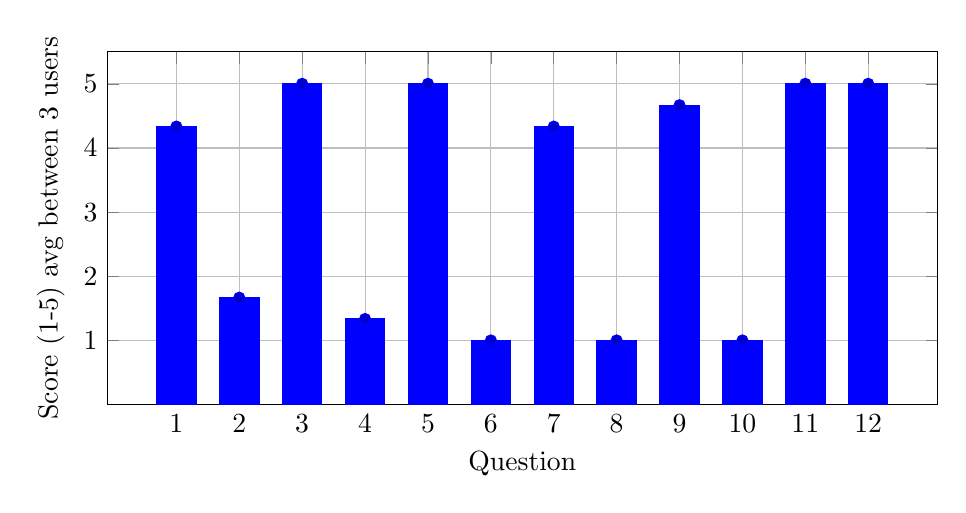
\begin{tikzpicture}
        \begin{axis}[
            width=\textwidth, 
            height=0.5\textwidth,
            xlabel=Question,
            ylabel=Score (1-5) avg between 3 users,
            ytick={1,2,3,4,5},
            xtick={1,2,3,4,5,6,7,8,9,10,11,12},
            ymin=0,
            % grid
            grid=both,
        ]
            \addplot+[ybar, fill=blue!, draw=blue!, bar width=0.5cm] coordinates {
                (1, 13/3)
                (2, 5/3)
                (3, 15/3)
                (4, 4/3)
                (5, 15/3)
                (6, 3/3)
                (7, 13/3)
                (8, 3/3)
                (9, 14/3)
                (10, 3/3)
                (11, 15/3)
                (12, 15/3)
            };
        \end{axis}
    \end{tikzpicture}
    \caption{The SUS questionnaire.}
    \label{fig:sus}
\end{figure}

The results of the SUS questionnaire are shown in \autoref{fig:sus}.
The average score for each question is computed by dividing the sum of the scores given by the 3 users by 3.
The SUS score can then be computed (ignoring the last two quesitons). 
The SUS scores are 95, 92.5 and 92.5, which leads to an average SUS score of 93.33, a pretty good score, considering that the SUS score is between 0 and 100.

The users also answered the two extra questions we added to the questionnaire that were more specific for a search engine.
The testers were very satisfied with the results of their queries, and they were able to complete all the tasks they were asked to do.

Given the results of the SUS questionnaire, we can say that the system is definitely usable and that the users are satisfied with it.


\section{How to run} \label{sec:howtorun}
The code of the system is available on GitHub at \url{https://github.com/Alessandro-Gobbetti/IR}.

To run the crawler, navigate to the \mintinline{bash}{crawler/crawler} folder and run:

\mintinline{bash}{scrapy crawl <spider-name> -o outputfile.json} (see \autoref{sec:crawling} for more info).

To init solr just navigate to the \mintinline{bash}{solr} folder and run \mintinline{bash}{make}.
This will start the solr instance on port 8983, creates a collection called \verb|creators| with the proper schema.
The MoreLikeThis handler is also added.

To start the backend, navigate to the \mintinline{bash}{backend} folder, install the dependencies with \mintinline{bash}{yarn install} and run \mintinline{bash}{yarn run start}.
By running \mintinline{bash}{yarn run solrinit} the backend clears the Solr collection and reindexes all the data.

To start the frontend, navigate to the \mintinline{bash}{frontend} folder, install the dependencies with \mintinline{bash}{yarn install} and run \mintinline{bash}{yarn run start}.



\section{Conclusion}

To conclude this report, we can say that we have successfully built a search engine for content creators on the internet.
The system is able to crawl the web and index the data, and it is able to perform queries and return the results to the user.
The backend automatically updates the data every $n$ days, so the user can always find the most up-to-date information about the artists.
The system is also able to recommend artists similar to the ones the user is interested in, and it is able to show the most popular tags.

The data retrieved are presented in a nice way to the user, and the user can easily interact with them expanding the cards
to see more information and clicking the links to the artists' pages.
The information shown are all the ones describin the artist, so in many cases the user does not even need to click on the link to the artist's page.

The user can also perform complex queries to find the artists that best fit their needs.
Since the crawling does not guarantee that all the artists are crawled, the user can also specify the query to be performed on the websites to improve the system.





\clearpage


\end{document}
